\documentclass{article}

\usepackage[english]{babel}
\usepackage{csquotes}
\usepackage[letterpaper,top=2cm,bottom=2cm,left=3cm,right=3cm,marginparwidth=1.75cm]{geometry}
\usepackage{listings}

\newcommand{\currentversion}{1.4}

\usepackage{amsmath}
\usepackage{graphicx}
\usepackage{biblatex}
\usepackage{float}
\usepackage{multirow}
\usepackage[colorlinks=true, allcolors=blue]{hyperref}

\graphicspath{{./assets}}
\addbibresource{references.bib}

\title{
\includegraphics[width=0.8\textwidth]{MINI.png} \\ Project of Application for Piano Music Generation \\ by Artificial Intelligence Algorithms \\ [0.35em]\large Laboratory No. 5, \\ Version \currentversion }
\author{}
\date{}

\begin{document}
\maketitle
\begin{center}
    \normalsize\textbf{Authors:}
    \vskip10pt
    \Large{Szymon Górski} \\
    \large{Index No. 298796}
    \vskip10pt
    \Large{Weronika Piotrowska} \\
    \large{Index No. 305793}
    \vskip10pt
    \Large{Marcin Wojnarowski} \\
    \large{Index No. 303880}
    \vskip50pt
    \normalsize\textbf{Thesis Supervisor:}
    \vskip10pt
    \Large{Jerzy Balicki} \\
    \large{DSc, Associate Professor}
    \vfill
    \large{Warsaw, 2022}
\end{center}

\newpage
\begin{abstract}
    This document outlines the bachelor thesis project for the last semester of Computer Science and Information Systems at the Faculty of Mathematics and Information Science Warsaw University of Technology. Project's technical documentation is hereby presented with installation instructions together with a usage manual.

    \hfill

    Previous documentations including detailed technical aspects and structures of the application can be found at \href{https://github.com/piotrowskv/music_generation/tree/main/docs}{https://github.com/piotrowskv/music\_generation/tree/main/docs} \label{previous_docs}
\end{abstract}

\vskip50pt
\section*{History of changes}
\begin{center}
    \begin{tabular}{ |p{0.07\textwidth} | p{0.1\textwidth} | p{0.5\textwidth} | p{0.21\textwidth}| }
        \hline
        Version & Date       & Description                                           & Author              \\
        \hline
        1.0     & 27.12.2022 & Initial document creation based on previous documents & Weronika Piotrowska \\
        \hline
        1.1     & 2.01.2023  & Added installation instructions                       & Szymon Górski       \\
        \hline
        1.2     & 2.01.2023  & Added deployment documentation                        & Weronika Piotrowska \\
        \hline
        1.3     & 3.01.2023  & Added technical documentation                         & Marcin Wojnarowski  \\
        \hline
        1.4     & 3.01.2023  & Added user manual                                     & Weronika Piotrowska \\
        \hline
    \end{tabular}
\end{center}

\newpage


\tableofcontents
\newpage

\section{Deployment Documentation}
% Requirements, Libraries, Hardware Resources, Configuration
\subsection{Hardware requirements}

Below, there are hardware requirements for running our application. The fact that machine learning is a computationally expensive task is directly visible in the presented requirements. Minimal machines will not suffice, though it is safe to assume it will work on most personal computers in 2023. Having an NVIDIA GPU will noticeably speed up model training.

\begin{enumerate}
    \item 64-bit operating system
    \item Processor (CPU): x86 or ARM architecture, at least 4 threads
    \item Memory (RAM): At least 4GB RAM
    \item Storage (disk space): At least 5GB disk space
    \item Input: Keyboard and mouse
    \item Optional, but strongly advised: NVIDIA GPU, GTX 650 or better
\end{enumerate}


\subsection{Software requirements} \label{software-deps} % languages, libraries, platforms, OS
We present software requirements for launching our application. This includes languages and libraries, but does not include Docker mentioned in Section \ref{installation}. After following the instruction, Docker will handle all languages and libraries dependencies, so there is no need to install points 2-7 separately.

\begin{enumerate}
    \item Any modern browser (Firefox, Chrome, Edge, Brave)
    \item Python version 3.10 \href{https://www.python.org/downloads/}{https://www.python.org/downloads/}
    \item pip 21.0.0 or newer \href{https://pypi.org/project/pip/}{https://pypi.org/project/pip/}
    \item pipenv 2022.3.23 or newer \href{https://pypi.org/project/pipenv/}{https://pypi.org/project/pipenv/}
    \item Python libraries: \textit{numpy} (1.23.5), \textit{keras} (2.10.0), \textit{tensorflow} (2.10.0), \textit{fastapi}, \textit{hypercorn}, \textit{mido}, \textit{music21}, \textit{websockets}, \textit{requests}

    \item Node.js 19.0.0 or newer \href{https://nodejs.org/en/}{https://nodejs.org/en/}
    \item JavaScript libraries: \textit{react} (18.2.0), \textit{typescript} (4.9.4), \textit{vite} (4.0.2), \textit{react-dom} (18.2.0), \textit{clsx} (1.2.1), \textit{react-router-dom} (6.5.0), \textit{ts-routes} (2.0), \textit{recharts} (2.2.0)
\end{enumerate}

\subsection{Configuration}

Since the application consists of a backend and frontend, there is a need for some configuration to establish their connection. Configuration options are kept minimal, to ease deployment.

\subsubsection{Port configuration}

Backend and frontend is free to work on any available port. To configure the running port for backend when starting it manually in the \verb|./backend| folder pass the binding flag to \verb|hypercorn|, example (binding to port 3030):

\verb|pipenv run hypercorn app.app --bind 0.0.0.0:3030|

To configure the port for frontend, when starting it manually in the \verb|./web| folder pass the port flag to \verb|vite|, example (binding to port 3030):

\verb|npm run dev -- --port 3030|


\subsubsection{Backend address configuration}

Frontend has to know where the backend is located. Therefore, there is a single environment variable called \verb|VITE_API_URL| which will point to the backend address. This variable will be read when building the application. Important, this address should not include the communication scheme. That is, instead of \verb|http://example.com/path| it should be just \verb|example.com/path|.

One can also edit the \verb|./web/.env| file to set the \verb|VITE_API_URL| environment variable.


\subsubsection{Docker configuration}

When running the application using docker instead of building manually, both ports and backend address are configured from the \verb|docker-compose.yml| file. To change the backend port modify \verb|services.backend.ports| by setting your preferred port. Similarly, to change the frontend port modify \verb|services.web.ports|. Example of setting the exposed port to 1234:

\begin{lstlisting}
ports:
  - 127.0.0.1:1234:80
\end{lstlisting}

To change the backend address modify \verb|services.web.build.args.VITE_API_URL|.


\section{Installation Instruction} \label{installation}
% What steps are needed to get it into production

The application is fully containerized using Docker, which means the whole project can be built by a single command while having only Docker installed.

In order to install and run the application, the following has to be done:

\begin{enumerate}
    \item Visit \href{https://github.com/piotrowskv/music_generation}{https://github.com/piotrowskv/music\_generation} and clone the code using \verb|git clone|.
    \item Download and install Docker \href{https://www.docker.com/}{https://www.docker.com/}
    \item In cloned repository, run \verb|docker compose up|
    \item Click on the port indicated by Docker to see the application (Fig. \ref{fig:docker})
\end{enumerate}

\begin{figure}[H]
    \centering
    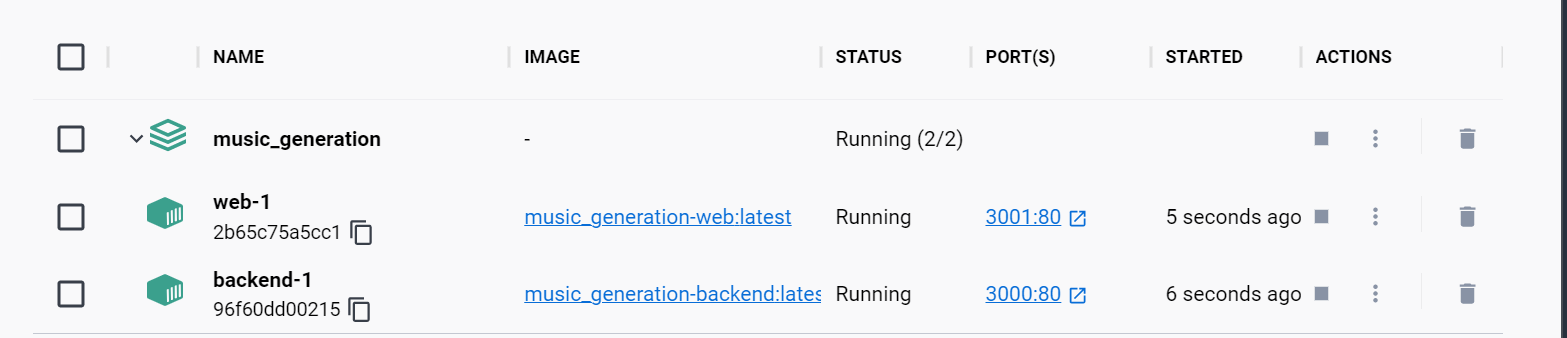
\includegraphics[width=0.7\textwidth]{assets/docker_sample.png}
    \caption{View of Docker after launching the application}
    \label{fig:docker}
\end{figure}

The project is now running and can be accessed in the browser by visiting the address \verb|http://localhost:3001|.


\subsection{Manual compilation}

Instead of using Docker, one can manually install all dependencies listed in Section \ref{software-deps}. Those steps will be now outlined. To run the backend, the following commands install libraries and build the server:

\begin{lstlisting}
    pipenv install
    pipenv run python main.py
\end{lstlisting}

To run the frontend, the following commands install lubraries and build the web server:

\begin{lstlisting}
    npm install
    npm run devd
\end{lstlisting}

\subsection{Deployed version}

The application has been built and deployed to be accessed online at \url{https://piotrowskv.github.io/music_generation}.

\section{Technical Documentation}
% Contracts of public interfaces and modules, Protocols
\subsection{System architecture}
The application consists of three following modules. The modules are designed so that replacing one module will not affect other modules.

\subsubsection{Models}
This module consists of pre-trained models (for details, see previous documentations), which can be also trained on datasets provided by the client. The main responsibilities of this module are:
\begin{itemize}
    \item Train and evaluate chosen model according to user's input
    \item Generate samples of music
    \item Change the training dataset to one provided by the user
    \item Adjust user's data to match model's input (for details, see previous documentations)
\end{itemize}

\subsubsection{Backend server}
The role of a backend server is to integrate between user and model. The main responsibilities of this module are:
\begin{itemize}
    \item Query models for training, evaluation and generation
    \item Answer client's queries
    \item Stream files from and to a client
    \item Save system logs
    \item Assert correct format of streamed files
\end{itemize}

\subsubsection{Frontend}
Frontend module will provide a GUI, which will allow the user to use the application. Its main responsibilities are:
\begin{itemize}
    \item Allow user to select, configure and train a model
    \item Allow user to upload own training dataset
    \item Allow user to download generated files
    \item Inform about model's training progress
    \item Display error messages
\end{itemize}

\subsection{Modules design}
\subsubsection{Layers}
We divide the application into two layers
\begin{itemize}
    \item Backend
    \item Frontend
\end{itemize}
The backend layer is responsible for implementing Model and API components. The frontend layer contains web application that will interact with the user.

\subsubsection{Dependencies}
Since the point of our application is to build and test Machine Learning models, there is no complicated dependencies between the classes. We define an abstract class \textit{MusicModel}, which then will be implemented by non-abstract classes. These classes will define certain model architecture. They will inherit methods and properties from the \textit{MusicModel} class, so that we can assure that they all are compatible with API (Backend) component. New architectures can be added in an easy way.

Backend component will consist of mainly API endpoint code, that is communication between chosen model and the client, thus it contains only sending and getting information methods. Described in more details in section \ref{sec:communication} and the attached OpenAPI specification (Attach. \ref{att:openapi}).



\subsection{Communication} \label{sec:communication} % protocols, libraries, network configuration

Our three components have a bidirectional linear communication flow, that is, each component talks with a single other component. Thus we differentiate the following communication schemes:

\subsubsection{Models \texorpdfstring{$\leftrightarrow$}{<->} Backend}

Since backend and models are just two different Python packages, the communication between them will happen through direct function calls. No special protocol is required here.

\subsubsection{Backend \texorpdfstring{$\leftrightarrow$}{<->} Frontend}

Here we distinguish two types of communication: request-response and real-time. In both cases the communication can be performed in a unsecure and a secure context. Respectively HTTP/HTTPS and WS/WSS.

\subsubsection{Request-Response}

For single request single response communication we will use the HTTP\footnote{HTTP -- Hypertext transfer protocol} protocol since it is the widely accepted protocol for the web. Our backend will support both HTTP/1.1 and HTTP/2 with the possibility to introduce HTTP/3 support (but not directly implemented by this project). For a meta-protocol REST\footnote{REST -- Representational state transfer} is a popular choice, and thus we will use it but with a small adjustment to adhere to the core CQRS\cite{CQRS}\footnote{CQRS -- Command-Query Responsibility Segregation} principle: queries should be idempotent and fetch some data (represented as HTTP's \texttt{GET} method), commands should modify some data but not return any (represented as HTTP's \texttt{POST} method). This simple modification allows for easier testing and maintainability.

In the attachments (Attach. \ref{att:openapi}) one can find the OpenAPI description of the API.

\subsubsection{Real-Time}

Some aspects will require real-time communication; that is, data can flow both ways without a need for instantiation through requests. For instance, when a model is being trained, backend will have to continuously push data to the frontend client about the current training status. In that case it is unreasonable to expect the client to ask for the newest training status all of the time. WebSockets fit this task perfectly. They allow for creating connections where both ends are able to push messages without any specific trigger.


These can be summarized in a single figure (Fig. \ref{fig:communication-diagram}).

\begin{figure}[H]
    \centering
    
\includegraphics[width=0.7\textwidth]{communication_diagram.png}
    \caption{Communication diagram for all three components. Arrow heads represent the direction of communication.}
    \label{fig:communication-diagram}
\end{figure}


\section{User's Manual}
% How to use the system
After installing and running the application as mentioned in Section \ref{installation}, the user is met with a starting screen as in Figure \ref{fig:app1}, where they can see a list of available models with a short description.

\begin{figure}[H]
    \centering
    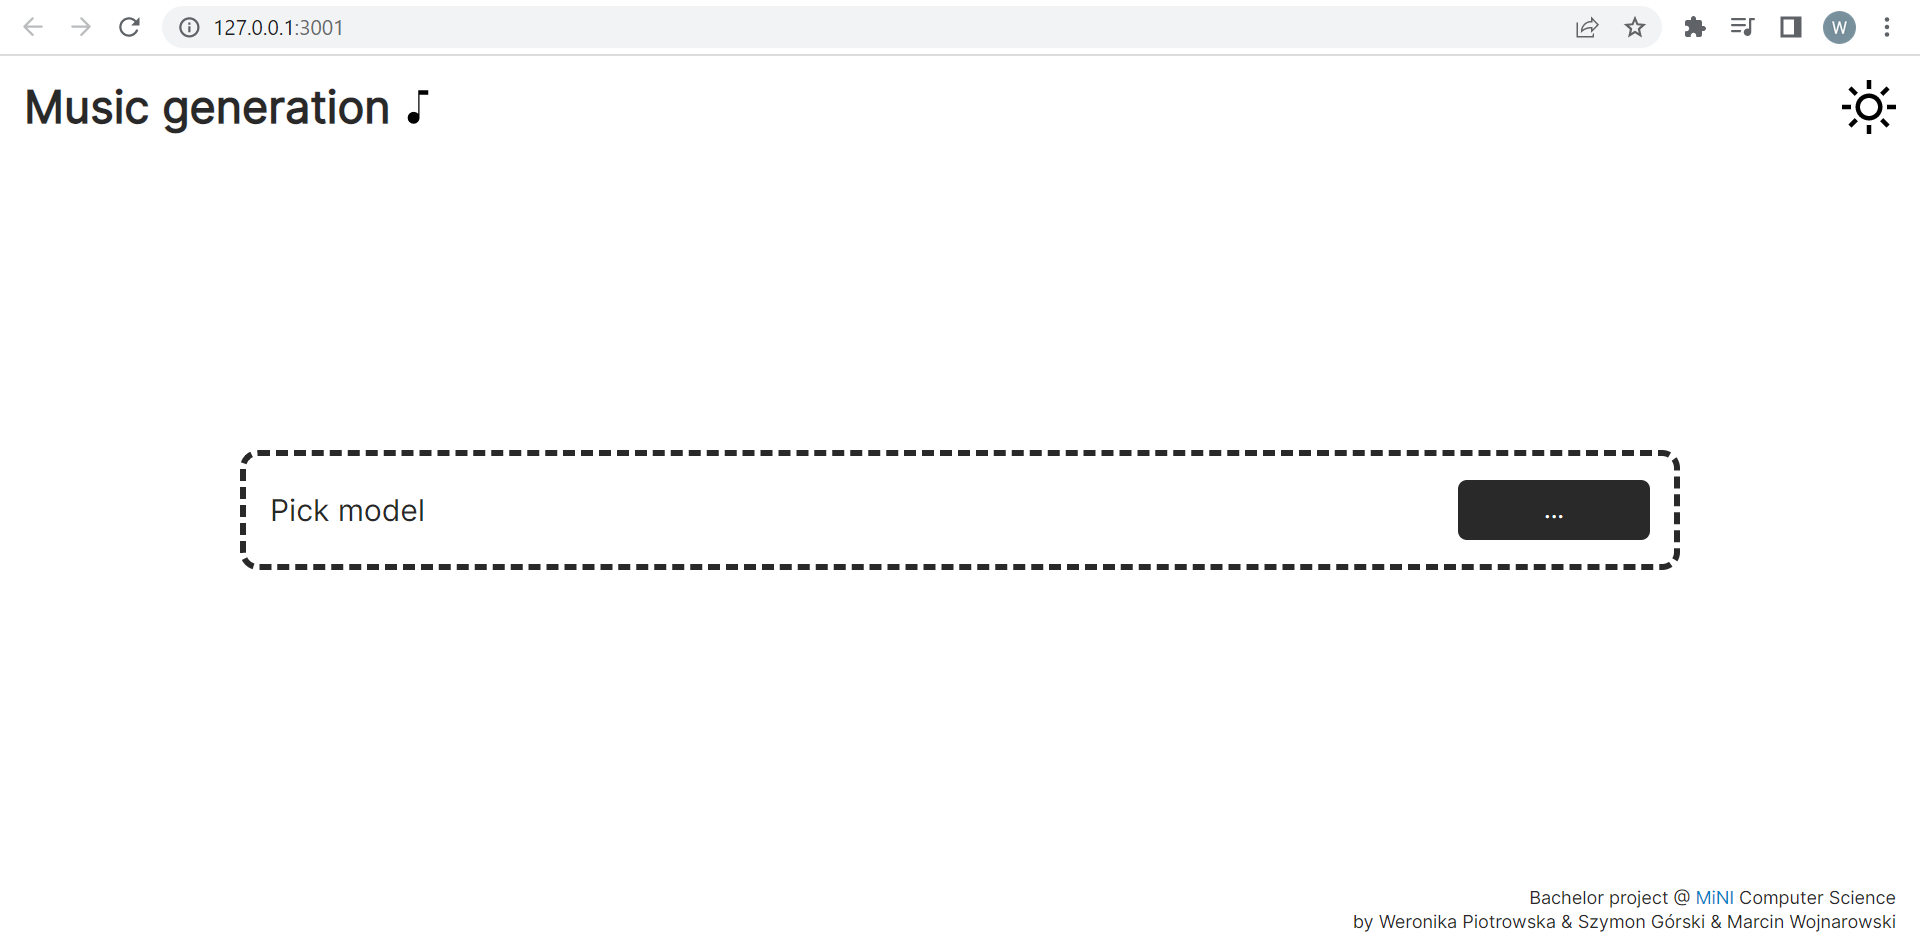
\includegraphics[width=0.7\textwidth]{assets/app1.png}
    \caption{Initial view of application}
    \label{fig:app1}
\end{figure}

After the user chooses a model, they will be instructed to choose either to use a pretrained model or train from scratch using own dataset. If the user chooses \textit{train myself}, then they can upload their own MIDI  files by providing them through a dialog or drag\&dropping them.

\begin{figure}[H]
    \centering
    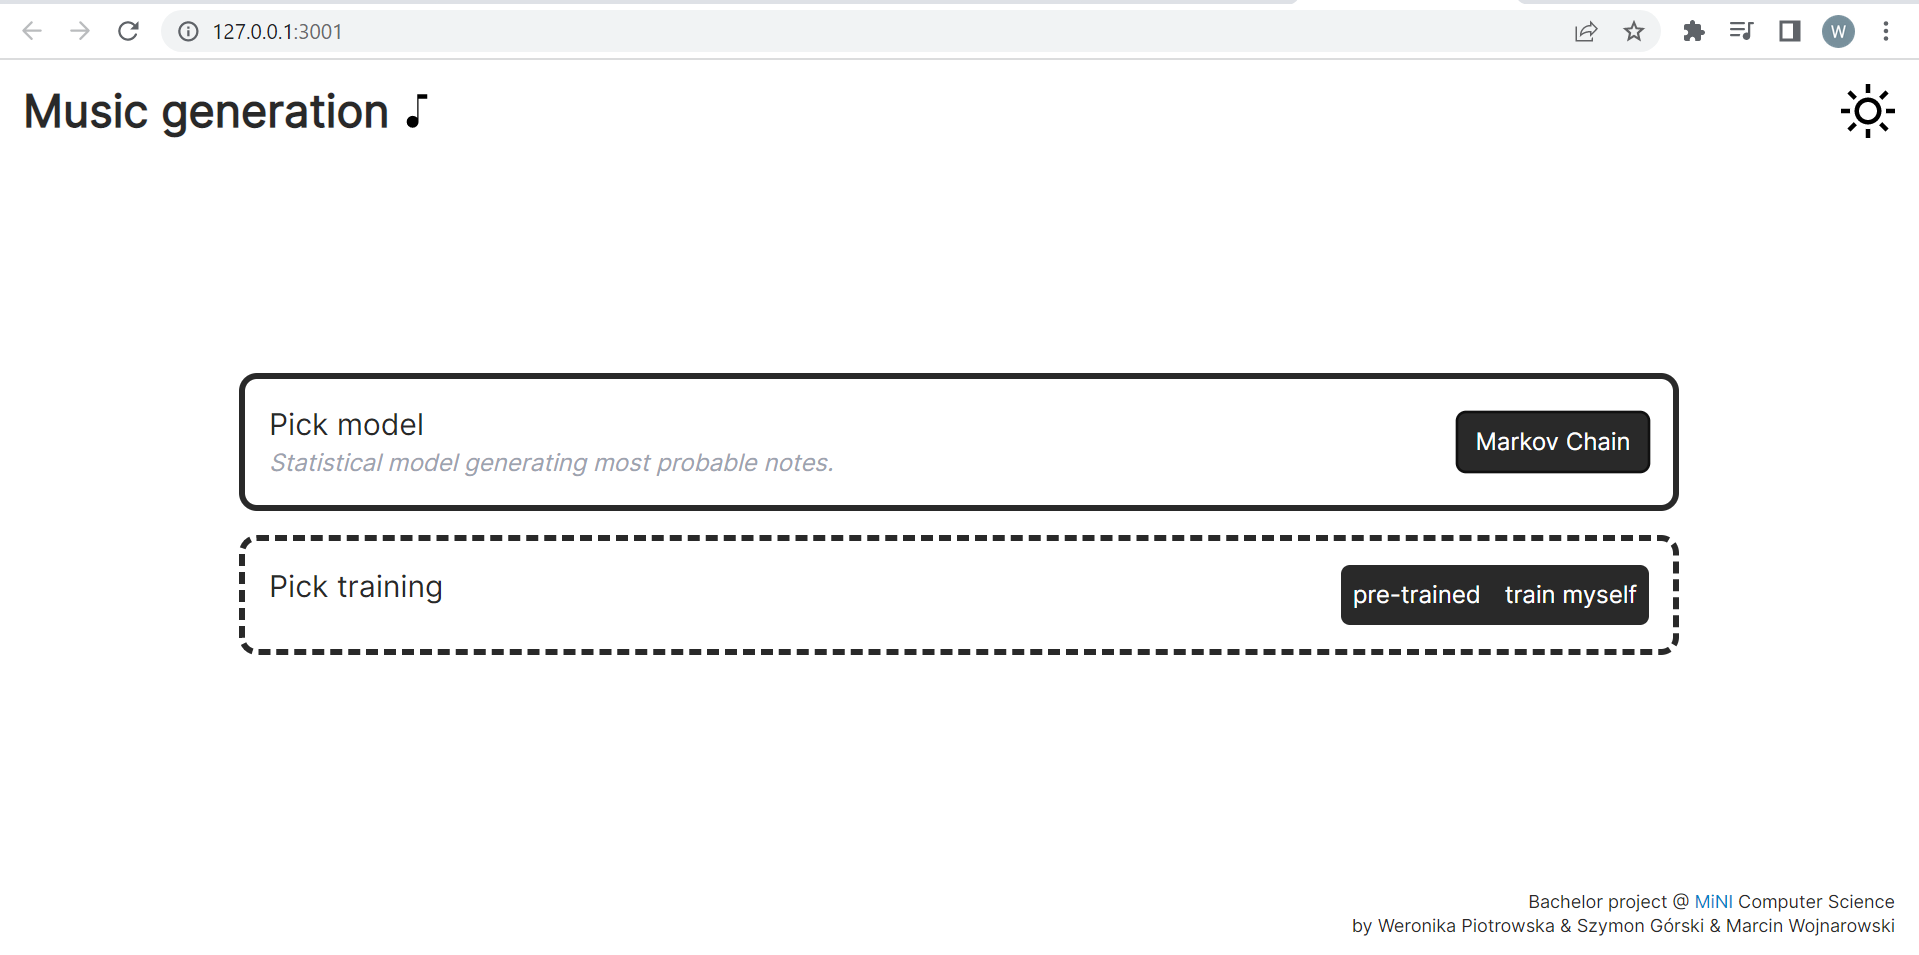
\includegraphics[width=0.7\textwidth]{assets/app2.png}
    \caption{Choice of training}
    \label{fig:app2}
\end{figure}

\begin{figure}[H]
    \centering
    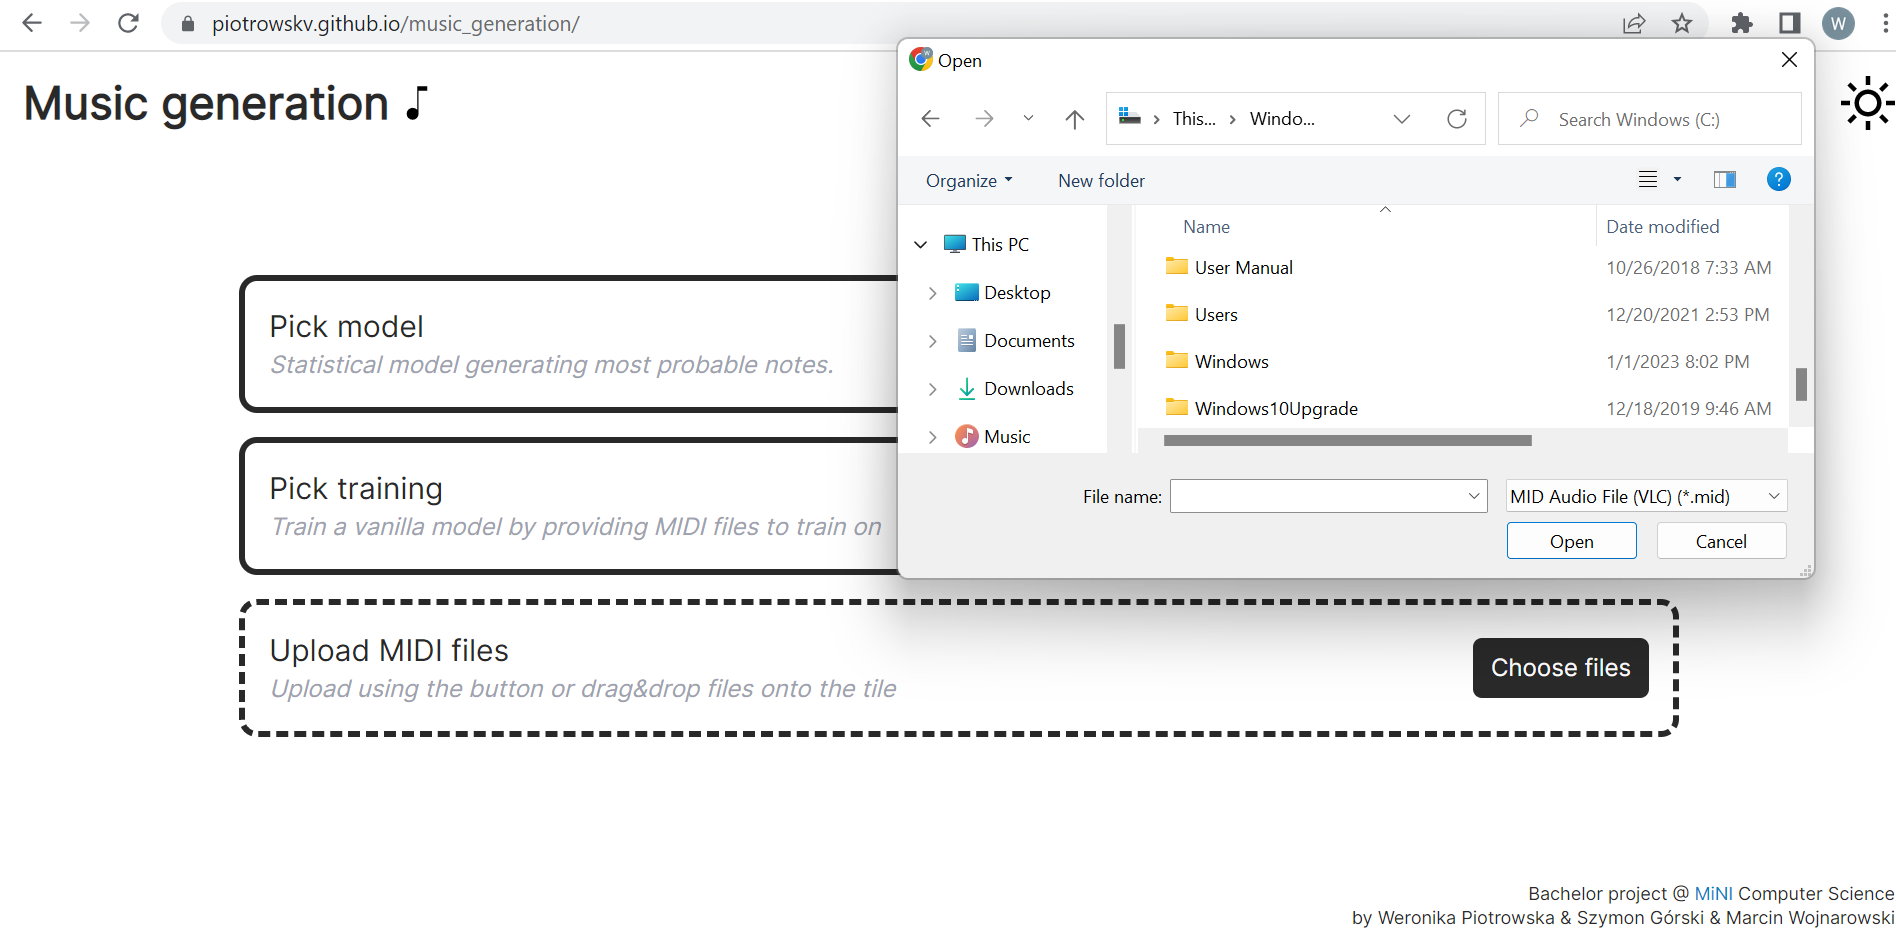
\includegraphics[width=0.7\textwidth]{assets/app3.png}
    \caption{Uploading files}
\end{figure}

After that, the training session is opened and the user is presented training statistics (loss, accuracy, or progress depending on the chosen model) of the model.

\begin{figure}[H]
    \centering
    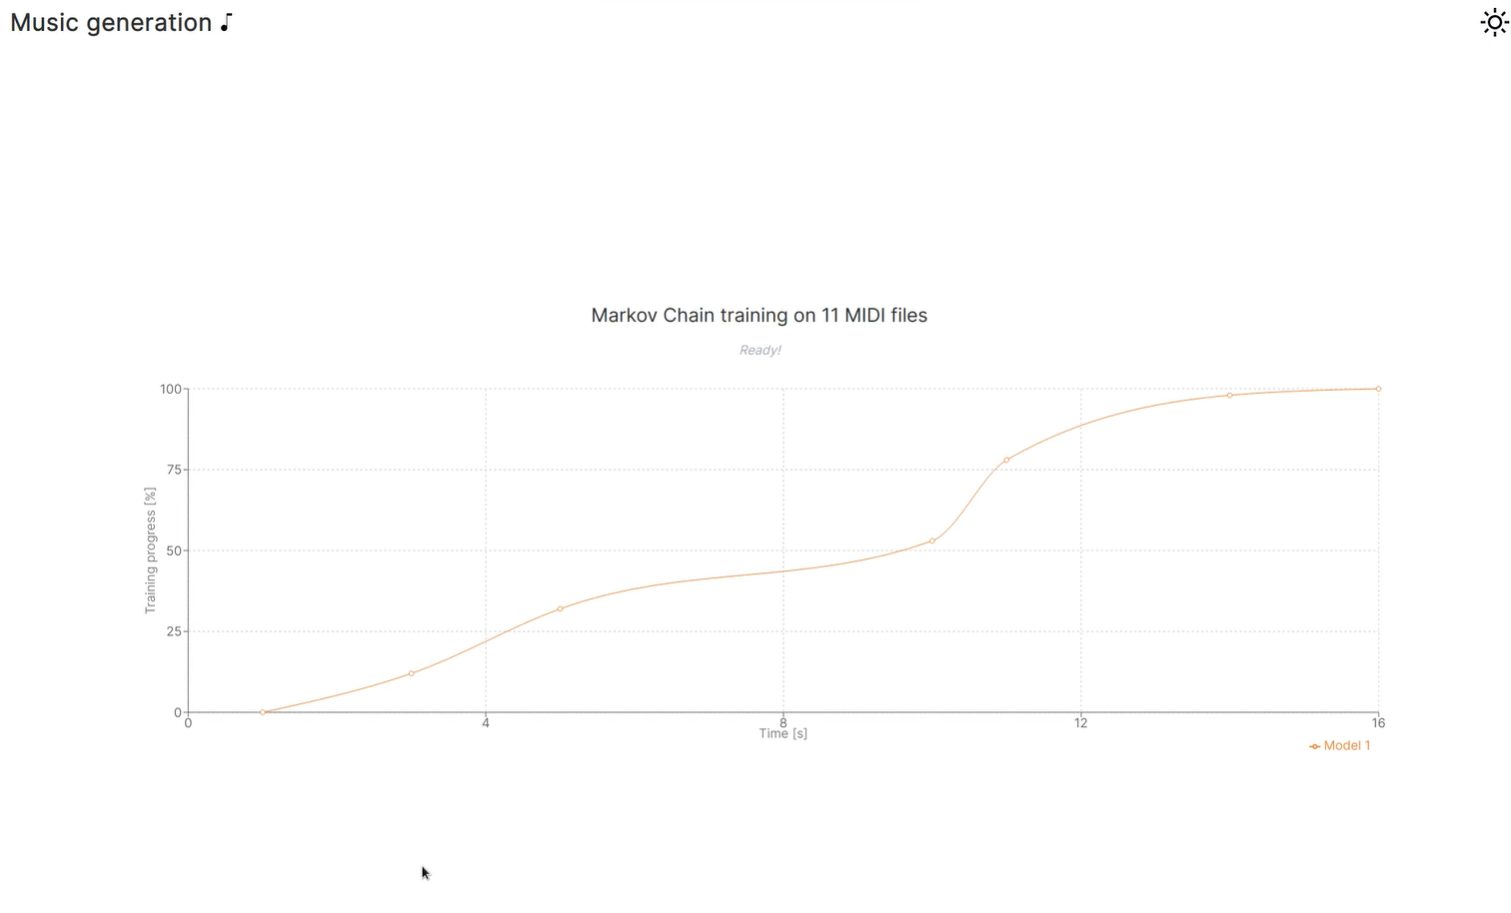
\includegraphics[width=0.7\textwidth]{assets/app4.png}
    \caption{Graph of model statistics}
\end{figure}
\newpage
\section{Attachments}

\begin{enumerate}
    \item \label{att:openapi} The OpenAPI description of the HTTP API
\end{enumerate}


\printbibliography


\end{document}
